% This contents of this file will be inserted into the _Solutions version of the
% output tex document.  Here's an example:

% If assignment with subquestion (1.a) requires a written response, you will
% find the following flag within this document: <SCPD_SUBMISSION_TAG>_1a
% In this example, you would insert the LaTeX for your solution to (1.a) between
% the <SCPD_SUBMISSION_TAG>_1a flags.  If you also constrain your answer between the
% START_CODE_HERE and END_CODE_HERE flags, your LaTeX will be styled as a
% solution within the final document.

% Please do not use the '<SCPD_SUBMISSION_TAG>' character anywhere within your code.  As expected,
% that will confuse the regular expressions we use to identify your solution.

\def\assignmentnum{1 }
\def\assignmentname{Sentiment Analysis}
\def\assignmenttitle{XCS221 Assignment \assignmentnum --- \assignmentname}
\input{macros}
\begin{document}
\pagestyle{myheadings} \markboth{}{\assignmenttitle}

% <SCPD_SUBMISSION_TAG>_entire_submission

This handout includes space for every question that requires a written response.
Please feel free to use it to handwrite your solutions (legibly, please).  If
you choose to typeset your solutions, the |README.md| for this assignment includes
instructions to regenerate this handout with your typeset \LaTeX{} solutions.
\ruleskip

\LARGE
1.e
\normalsize

% <SCPD_SUBMISSION_TAG>_1e
\begin{answer}
  % ### START CODE HERE ###
Question: Run your linear predictor with feature extractor extractCharacterFeatures. Experiment with different values of
n to see which one produces the smallest test error. You should observe that this error is nearly as small as
that produced by word features. Why is this the case?

Answer: Experiment conducted with values of n ranging from 1 to 15 showed that test error decreased
as n increased from 1 to 5, stayed low between 5 to 7 (lowest being at 7) and started to increase for n between 7 and 15.

Also, it was found that low test errors which were found for n between 5 and 7 was nearly as small as that 
produced by word features. This is because most of the words in English language are expected to have their length 
around 5 to 7 characters. And at this length, character n-grams are able to capture the complete words (atleast the 
ones which contribute meaningfully as predictors) from movie reviews and hence, provide similar performance as word features.


\begin{figure}
  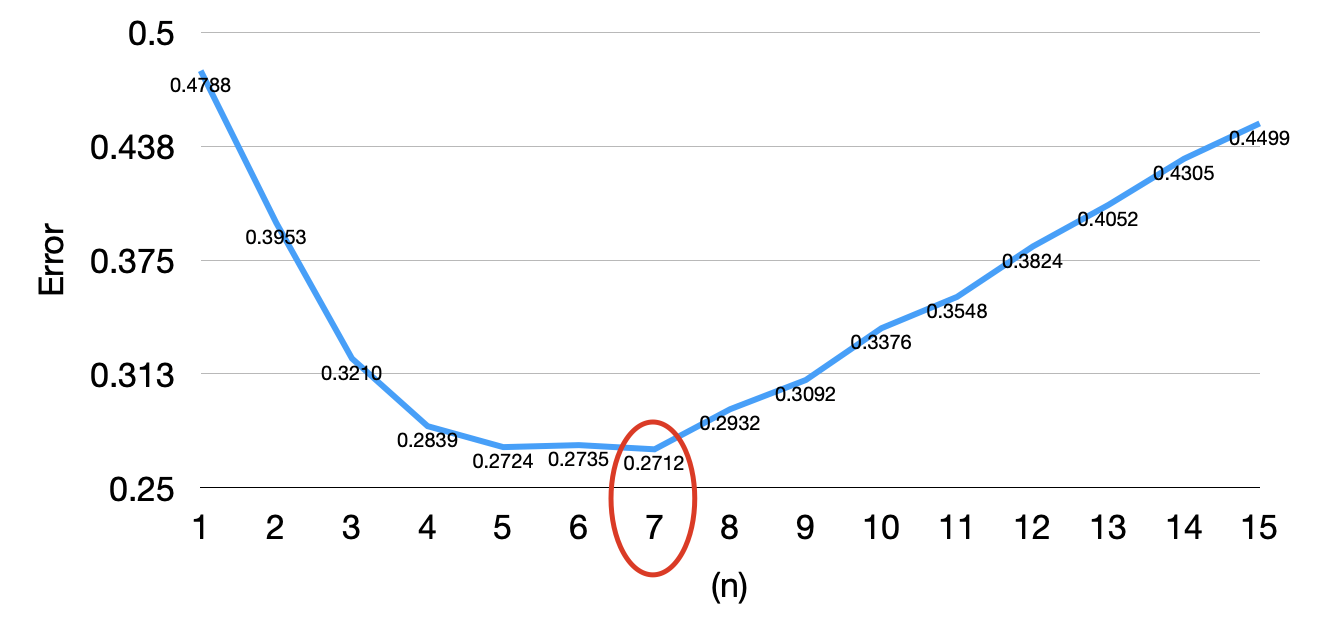
\includegraphics[width=\linewidth]{images/1e_error_graph.png}
  \caption{Error vs n-gram features.}
  \label{fig:error_graph}
\end{figure}

<<
Below is the result for word features based model:
Epoch 20: Train Error = 0.027011817670230726, Validation Error = 0.27124366910523356
>>
<<
Below are the results for different values of n (character n-grams):
Testing for n = 1
Official: train error = 0.45723128868880136, validation error = 0.47889701744513224

Testing for n = 2
Official: train error = 0.2839054586381542, validation error = 0.3953292065278559

Testing for n = 3
Official: train error = 0.0025323579065841305, validation error = 0.32104670793472145

Testing for n = 4
Official: train error = 0.0, validation error = 0.2839054586381542

Testing for n = 5
Official: train error = 0.0, validation error = 0.2723691615081598

Testing for n = 6
Official: train error = 0.0, validation error = 0.2734946539110861

Testing for n = 7
Official: train error = 0.0002813731007315701, validation error = 0.27124366910523356

Testing for n = 8
Official: train error = 0.0005627462014631402, validation error = 0.293190770962296

Testing for n = 9
Official: train error = 0.0008441193021947102, validation error = 0.3092290377039955

Testing for n = 10
Official: train error = 0.0008441193021947102, validation error = 0.3376477208778841

Testing for n = 11
Official: train error = 0.0008441193021947102, validation error = 0.35481148002250984

Testing for n = 12
Official: train error = 0.0008441193021947102, validation error = 0.3823860438942037

Testing for n = 13
Official: train error = 0.0016882386043894203, validation error = 0.4051772650534609

Testing for n = 14
Official: train error = 0.0022509848058525606, validation error = 0.4305008441193022

Testing for n = 15
Official: train error = 0.0028137310073157004, validation error = 0.44991558806978055
>>
-------
Question: Construct a review (one sentence max) in which character n-grams probably outperform word features, and
briefly explain why this is so.

Answer: Let's look at 2 reviews to understand when 'character n-grams' outperforms 'word features':
Here is an example of negative movie review (label = -1): 'Acting is bad , story is not good'.
Here is an example of positive movie review (label = +1): 'Acting is good , story is not bad'.

'character n-grams (n=7)' based model is able to correctly classify both the examples
because 'character 7-grams' allows it to capture the fact that 'not good' is a negative phrase and 'not bad' is positive.

However, 'word features' based model fails to capture this nuance and classifies the positive review incorrectly. It
considered both the examples to be same because the model treated 'not' as a separate feature and failed to capture the
importance of its positioning.

Testing these examples using both feature extractors provided below mentioned outcomes (as expected):
<<
Testing with extractCharacterFeatures(n=7):
Correctly classified review example ['Acting is good , story is not bad', 1] as 1 with margin 0.010000000000000004
Correctly classified review example ['Acting is bad , story is not good', -1] as -1 with margin 0.03

Testing with extractWordFeatures():
Incorrectly classified review example ['Acting is good , story is not bad', 1] as -1 with margin -0.40000000000000147
Correctly classified review example ['Acting is bad , story is not good', -1] as -1 with margin 0.4000000000000014
>>
  % ### END CODE HERE ###
\end{answer}
% <SCPD_SUBMISSION_TAG>_1e
\clearpage

\LARGE
2.a
\normalsize

% <SCPD_SUBMISSION_TAG>_2a
\begin{answer}
  % ### START CODE HERE ###
  % ### END CODE HERE ###
\end{answer}
% <SCPD_SUBMISSION_TAG>_2a
\clearpage

% <SCPD_SUBMISSION_TAG>_entire_submission
\end{document}